\documentclass[conference]{IEEEtran}

% ---------- Packages ----------
\usepackage{newtxtext,newtxmath} % Times系/数式
\usepackage{amsmath}
\usepackage{siunitx}
\usepackage{graphicx,xcolor}
\usepackage{booktabs}
\usepackage{placeins}
\usepackage[hidelinks]{hyperref}
\usepackage{tikz}
\usetikzlibrary{calc,positioning,fit,arrows.meta,shapes.geometric,shapes.misc}

% ---------- TikZ styles ----------
\tikzset{
  line/.style={-Latex, line width=0.45pt},
  box/.style={draw, rounded corners, align=center, inner sep=3pt},
  smallbox/.style={box, minimum width=26mm, minimum height=6mm},
  midbox/.style={box, minimum width=32mm, minimum height=7mm},
  bigbox/.style={box, minimum width=66mm, minimum height=8mm},
  % for Fig.1 flow (片欄)
  step/.style={box, minimum width=31mm, minimum height=7mm}
}

% ---------- Title ----------
\title{AITL on Space: A Robust Three-Layer Architecture\\
with a Tri-NVM Hierarchy (SRAM / MRAM / FRAM)\\
for Long-Duration Spacecraft Autonomy}

\author{
\IEEEauthorblockN{Shinichi Samizo}
\IEEEauthorblockA{Independent Semiconductor Researcher\\
Former Engineer at Seiko Epson Corporation\\
Email: shin3t72@gmail.com\quad GitHub: \url{https://github.com/Samizo-AITL}}
}

\begin{document}
\maketitle

\begin{abstract}
We propose \emph{AITL on Space}, a three-layer control architecture (Robust Core, FSM Supervisor, AI Adaptor) integrated with a tri-NVM hierarchy (SRAM/MRAM/FRAM) and mapped to a 22\,nm FD\!SOI SoC. The contribution is a complete end-to-end design flow from mission-level specification to ASIC: requirements are formalized as JSON via \emph{EduController}, synthesized by the \emph{AITL-H} module, validated in FPGA HIL with fault injection, stress-tested through \emph{SystemDK FEM} (thermal/radiation/packaging), and finally implemented as ASIC. This methodology enables resilient autonomy for long-duration spacecraft missions.
\end{abstract}

\section{Introduction}
Deep-space missions require ultra-robust control under total ionizing dose (TID), single event effects (SEE), and thermal cycling. Conventional PID+Flash architectures face lifetime limits due to charge-trap drift and endurance. We present \emph{AITL on Space}: a resilient three-layer architecture with a tri-NVM hierarchy and a reproducible design flow from specification to ASIC.

\section{Specification and Design Flow}
The process begins with \emph{Mission Specification}. Requirements such as pointing accuracy, power stability, and thermal tolerance are captured in \emph{EduController}, a model-based tool that exports plant matrices and weighting functions as JSON (portable across simulators). The JSON is consumed by \emph{AITL-H}, which synthesizes an $H_\infty$ output-feedback controller $K$ with mixed-sensitivity weighting and generates a fixed-point implementation for RTL/FPGA/ASIC. The design then undergoes:
\begin{itemize}
  \item \textbf{FPGA HIL}: hardware-in-the-loop validation with SEU \& outage injection; metrics include safe-mode entry $<\!1$\,s, recovery rate $\ge\!99\%$, and ECC scrubbing efficiency.
  \item \textbf{SystemDK FEM}: co-simulation of thermal cycles, radiation effects, and packaging stress, closing the verification loop before silicon.
  \item \textbf{ASIC Mapping}: implementation on GlobalFoundries 22FDX FD\!SOI hardened for long-duration missions.
\end{itemize}

\textit{Toolchain at a Glance}. \emph{EduController}=\textit{spec-to-JSON exporter} (plant $A,B,C,D$, noise/disturbance models, weights $W_1,W_2,W_3$). \emph{AITL-H}=$H_\infty$ synthesizer (Riccati/\!LMI$\rightarrow$ fixed-point $K$ with range/scaling for RTL). \emph{SystemDK FEM}=\textit{physics closer} (thermal/radiation/packaging) used to derate timing/power and validate memory scrubbing.

\section{System Architecture}
AITL consists of three layers:
\begin{itemize}
  \item \textbf{Robust Core}: $H_\infty$/MPC/SMC controllers for ultra-robust stability.
  \item \textbf{FSM Supervisor}: mode switching (Safe/Nominal/Recovery) with FDI/FDII for fault management.
  \item \textbf{AI Adaptor}: long-term re-identification and drift compensation.
\end{itemize}
The tri-NVM hierarchy ensures persistence: SRAM for execution, MRAM for logs/code with ECC scrubbing and dual slots, and FRAM for safe boot and FSM states. Target SoC is 22\,nm FD\!SOI hardened for radiation and temperature stress.

\section{Mathematical Model and $H_\infty$ Design}
We consider an 11D discrete-time state-space plant coupling attitude (6), power bus (2), and thermal nodes (3):
\begin{align}
  x_{k+1} &= A x_k + B u_k + E w_k, \label{eq:ss1}\\
  y_k &= C x_k + D u_k + v_k, \label{eq:ss2}
\end{align}
where $w_k$ and $v_k$ denote disturbance and noise. The model extends to 20D by adding translational axes and bias states. Weights $(W_1,W_2,W_3)$ shape sensitivity, control effort, and complementary sensitivity. \emph{EduController} outputs them as JSON; \emph{AITL-H} synthesizes $K$ with robustness margins, mapped to fixed-point for RTL/FPGA/ASIC.

\section{Verification Pipeline}
FPGA HIL injects SEUs and sensor outages. Metrics include safe-mode entry time ($<\!1$\,s), recovery rate ($\ge\!99\%$), and ECC scrubbing efficiency. \emph{SystemDK FEM} validates thermal and radiation stress, ensuring packaging reliability before ASIC tape-out.

\section{Conclusion}
AITL on Space combines robust control, supervisory safety, AI re-identification, and hardened memory. The proposed end-to-end flow—from mission specification to ASIC—provides a reproducible methodology for resilient autonomy in long-duration space missions.

% ---------- References ----------
\begin{thebibliography}{99}
\bibitem{doyle}
J.\,C.~Doyle, B.\,A.~Francis, and A.\,R.~Tannenbaum,
\emph{Feedback Control Theory}. Macmillan, 1992.

\bibitem{colinge}
J.-P.~Colinge, \emph{Silicon-on-Insulator Technology: Materials to VLSI}, 3rd~ed. Springer, 2004.

\bibitem{wolf}
W.~Wolf, \emph{FPGA-Based System Design}. Prentice Hall, 2004.

\bibitem{rabaey}
J.~M.~Rabaey, A.~Chandrakasan, and B.~Nikoli\'c,
\emph{Digital Integrated Circuits: A Design Perspective}, 2nd~ed. Prentice Hall, 2003.
\end{thebibliography}

% ---------- Biography ----------
\section*{Author Biography}
Shinichi Samizo received the M.S.\ degree in Electrical and Electronic Engineering from Shinshu University, Japan. He worked at Seiko Epson Corporation as an engineer in semiconductor memory and mixed-signal device development, and contributed to inkjet MEMS actuators and PrecisionCore printhead technology. He is currently an independent semiconductor researcher focusing on process/device education, memory architecture, and AI system integration. Contact: \texttt{shin3t72@gmail.com}.

% =========================================================
% Figures are collected at the very end:
%   Fig.1 and Fig.3 = single-column
%   Fig.2            = double-column (across both columns)
% =========================================================

\section*{Figures}

% ---------- Fig.1 (single column) ----------
\begin{figure}[!t]
\centering
\begin{tikzpicture}[node distance=4.5mm, scale=0.96, every node/.style={transform shape}]
  \node[step, fill=purple!10] (spec) {Mission Specification};
  \node[step, fill=blue!10, below=of spec] (json) {EduController JSON Export};
  \node[step, fill=green!12, below=of json] (hinf) {AITL-H $H_\infty$ Synthesis};
  \node[step, fill=orange!18, below=of hinf] (hil) {FPGA HIL Verification};
  \node[step, fill=red!10, below=of hil] (asic) {22FDX ASIC Implementation};
  \node[step, fill=cyan!12, right=18mm of hil] (fem) {\shortstack{SystemDK FEM\\Thermal / Radiation / Packaging}};
  \draw[line] (spec) -- (json) -- (hinf) -- (hil) -- (asic);
  \draw[line] (hinf.east) -| (fem.north);
  \draw[line] (hil.east)  -- ++(6mm,0) |- (fem.west);
\end{tikzpicture}
\caption{End-to-end flow: Mission Spec $\rightarrow$ JSON (EduController) $\rightarrow$ AITL-H $\rightarrow$ FPGA HIL $\rightarrow$ FEM $\rightarrow$ ASIC.}
\label{fig:flow}
\end{figure}

% ---------- Fig.2 (double column, orthogonal配線) ----------
\begin{figure*}[!t]
\centering
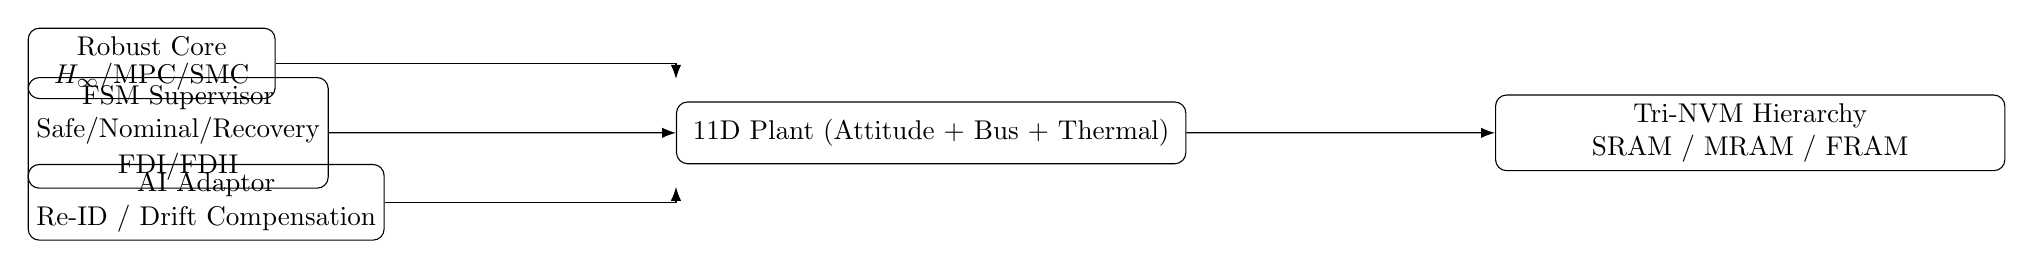
\begin{tikzpicture}[node distance=7mm, scale=0.98, every node/.style={transform shape}]
  \node[midbox, anchor=west] (core) at (0,0.8) {\shortstack{Robust Core\\$H_\infty$/MPC/SMC}};
  \node[midbox, below=9mm of core.west, anchor=west] (fsm) {\shortstack{FSM Supervisor\\Safe/Nominal/Recovery\\FDI/FDII}};
  \node[midbox, below=9mm of fsm.west, anchor=west] (ai) {\shortstack{AI Adaptor\\Re-ID / Drift Compensation}};
  \node[bigbox, right=45mm of fsm] (plant) {11D Plant (Attitude + Bus + Thermal)};
  \node[bigbox, right=40mm of plant] (nvm)   {\shortstack{Tri-NVM Hierarchy\\SRAM / MRAM / FRAM}};
  % orthogonal wiring
  \draw[line] (core.east) -| ($(plant.west)+(0,7mm)$);
  \draw[line] (fsm.east) -- (plant.west);
  \draw[line] (ai.east)  -| ($(plant.west)+(0,-7mm)$);
  \draw[line] (plant.east) -- (nvm.west);
\end{tikzpicture}
\caption{AITL architecture: three control layers with tri-NVM memory hierarchy. Orthogonal interconnects (no diagonal lines) improve readability.}
\label{fig:arch}
\end{figure*}

% ---------- Fig.3 (single column) ----------
\begin{figure}[!t]
\centering
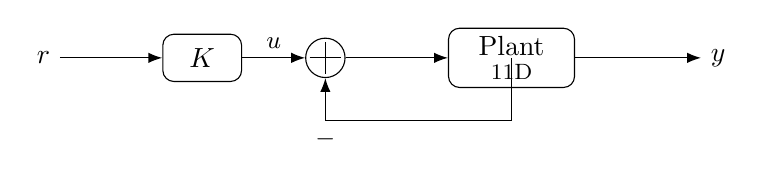
\begin{tikzpicture}[node distance=9mm]
  \node[smallbox, minimum width=10mm] (K) {$K$};
  \node[circle, draw, minimum size=5mm, right=8mm of K] (sum) {};
  \draw (sum) +(-2mm,0) -- +(2mm,0);
  \draw (sum) +(0,-2mm) -- +(0,2mm);
  \node[smallbox, right=13mm of sum, minimum width=16mm] (P) {\shortstack{Plant\\\footnotesize 11D}};
  \node[right=16mm of P] (y) {$y$};
  \node[left=13mm of K] (r) {$r$};
  \draw[line] (r) -- (K);
  \draw[line] (K) -- node[above]{\small $u$} (sum);
  \draw[line] (sum) -- (P);
  \draw[line] (P) -- (y);
  \draw[line] ($(P.north)!0.5!(P.south)$) |- ++(0,-8mm) -| node[below]{\small $-$} (sum.south);
\end{tikzpicture}
\caption{Closed-loop system for $H_\infty$ mixed-sensitivity synthesis on the 11D plant.}
\label{fig:loop}
\end{figure}

% 2ページ完結に近づけるためのヒント(必要なら有効化)
% \IEEEtriggeratref{3} % 参考文献の途中でコラム長をそろえる際に使用
% \IEEEtriggercmd{\enlargethispage{-1.1\baselineskip}}

\end{document}
